\clearpage
\section*{September 14, 2026: First joint-model fit with a flat charge}
\textit{Agent-drafted research entry. Numerical exhibits are frozen at the
September 22 build preceding the historical source correction; they are not
estimates from the corrected 23Q4 panel. The original experiment is described below.}
\newcommand{\NotchKappa}{0.11}
\newcommand{\NotchSigma}{1.1}
\newcommand{\NotchMean}{149.8}
\newcommand{\NotchObservedMean}{136.6}
\newcommand{\NotchUnitLoss}{495}
\newcommand{\NotchDirectGap}{4587}
\newcommand{\NotchReorganizationUnits}{92}
\newcommand{\NotchShareNinetyNine}{12.6}
\newcommand{\NotchSharePairs}{4.4}
\newcommand{\NotchShareThreePlus}{12.3}
\newcommand{\NotchShareDoubleNinetyNine}{0.19}


The first pure-notch pilot matches the overall 99-unit spike but misses how
parents organize into filings. Jacob requested a first estimation with the
marginal-cost parameter fixed at $\tau=0$. The baseline uses quadratic ordinary
size loss, $((m-x)/99)^2$, and separate assessment of each constituent. Its
best searched values are $\kappa=\NotchKappa$ and
$\sigma_{\mathrm{org}}=\NotchSigma$, in normalized profit-scale units.

The counterfactual is the joint distribution of total units and constituent
counts among 561 historical rental parents from 2019--2022, using the saved
site weights. The target comprises 316 rental parents from January 2025 through
July 8, 2026. Both samples require at least 50 units and composition eligibility.
Weights balance log lot area, residential FAR, built FAR, and borough.
The parent land footprint is taken as given. Housing Database units retain
priority with DOB fallback, and each selected parent vector is checked against
the additive constituent panel.

Each historical parent's original constituent count has zero ordinary
disadvantage. Other counts independently draw exponential disadvantages with
mean $\sigma_{\mathrm{org}}$. Every parent can choose one through six positive-size
constituents within its given footprint. Estimation minimizes equally weighted
squared share errors in 15 disjoint size bins crossed with one, two, or three-plus
constituents. This fits joint masses; it does not estimate a cutoff from the
first observed project above 99.

\begin{center}
\begin{tabular}{lrr}
\hline
Outcome & Observed post & Fitted baseline \\
\hline
Parents at 99 units (\%) & 12.3 & \NotchShareNinetyNine \\
Exactly two constituents (\%) & 12.7 & \NotchSharePairs \\
Three or more constituents (\%) & 3.5 & \NotchShareThreePlus \\
Parents organized as $99+99$ (\%) & 2.85 & \NotchShareDoubleNinetyNine \\
Mean proposed units & \NotchObservedMean & \NotchMean \\
\hline
\end{tabular}
\end{center}

The model implies \NotchUnitLoss{} fewer proposed units across 316 parents;
the difference between the reweighted historical and observed post totals is
\NotchDirectGap{} units. Reorganization preserves \NotchReorganizationUnits{}
units relative to holding historical constituent counts fixed while allowing
size and layout to adjust. These comparisons condition on the number of parents.
The unexplained difference can reflect model or counterfactual misspecification;
it does not identify compression, entry, or completed housing separately.

The organization pattern exposes a consequential assumption. Once a count makes
a parent exempt, still larger counts offer the same policy saving. Independent
cost draws with the same mean spread choices over these counts. The next model
question is how the cost of adding one filing differs from adding several.
An unrestricted layout also permits one large constituent to absorb all taxed
units. Four observed parents have multiple 100-plus constituents, warranting a
comparison with site feasibility and legal assessment before treating this
feature as a direct rejection.

\clearpage
\begin{center}
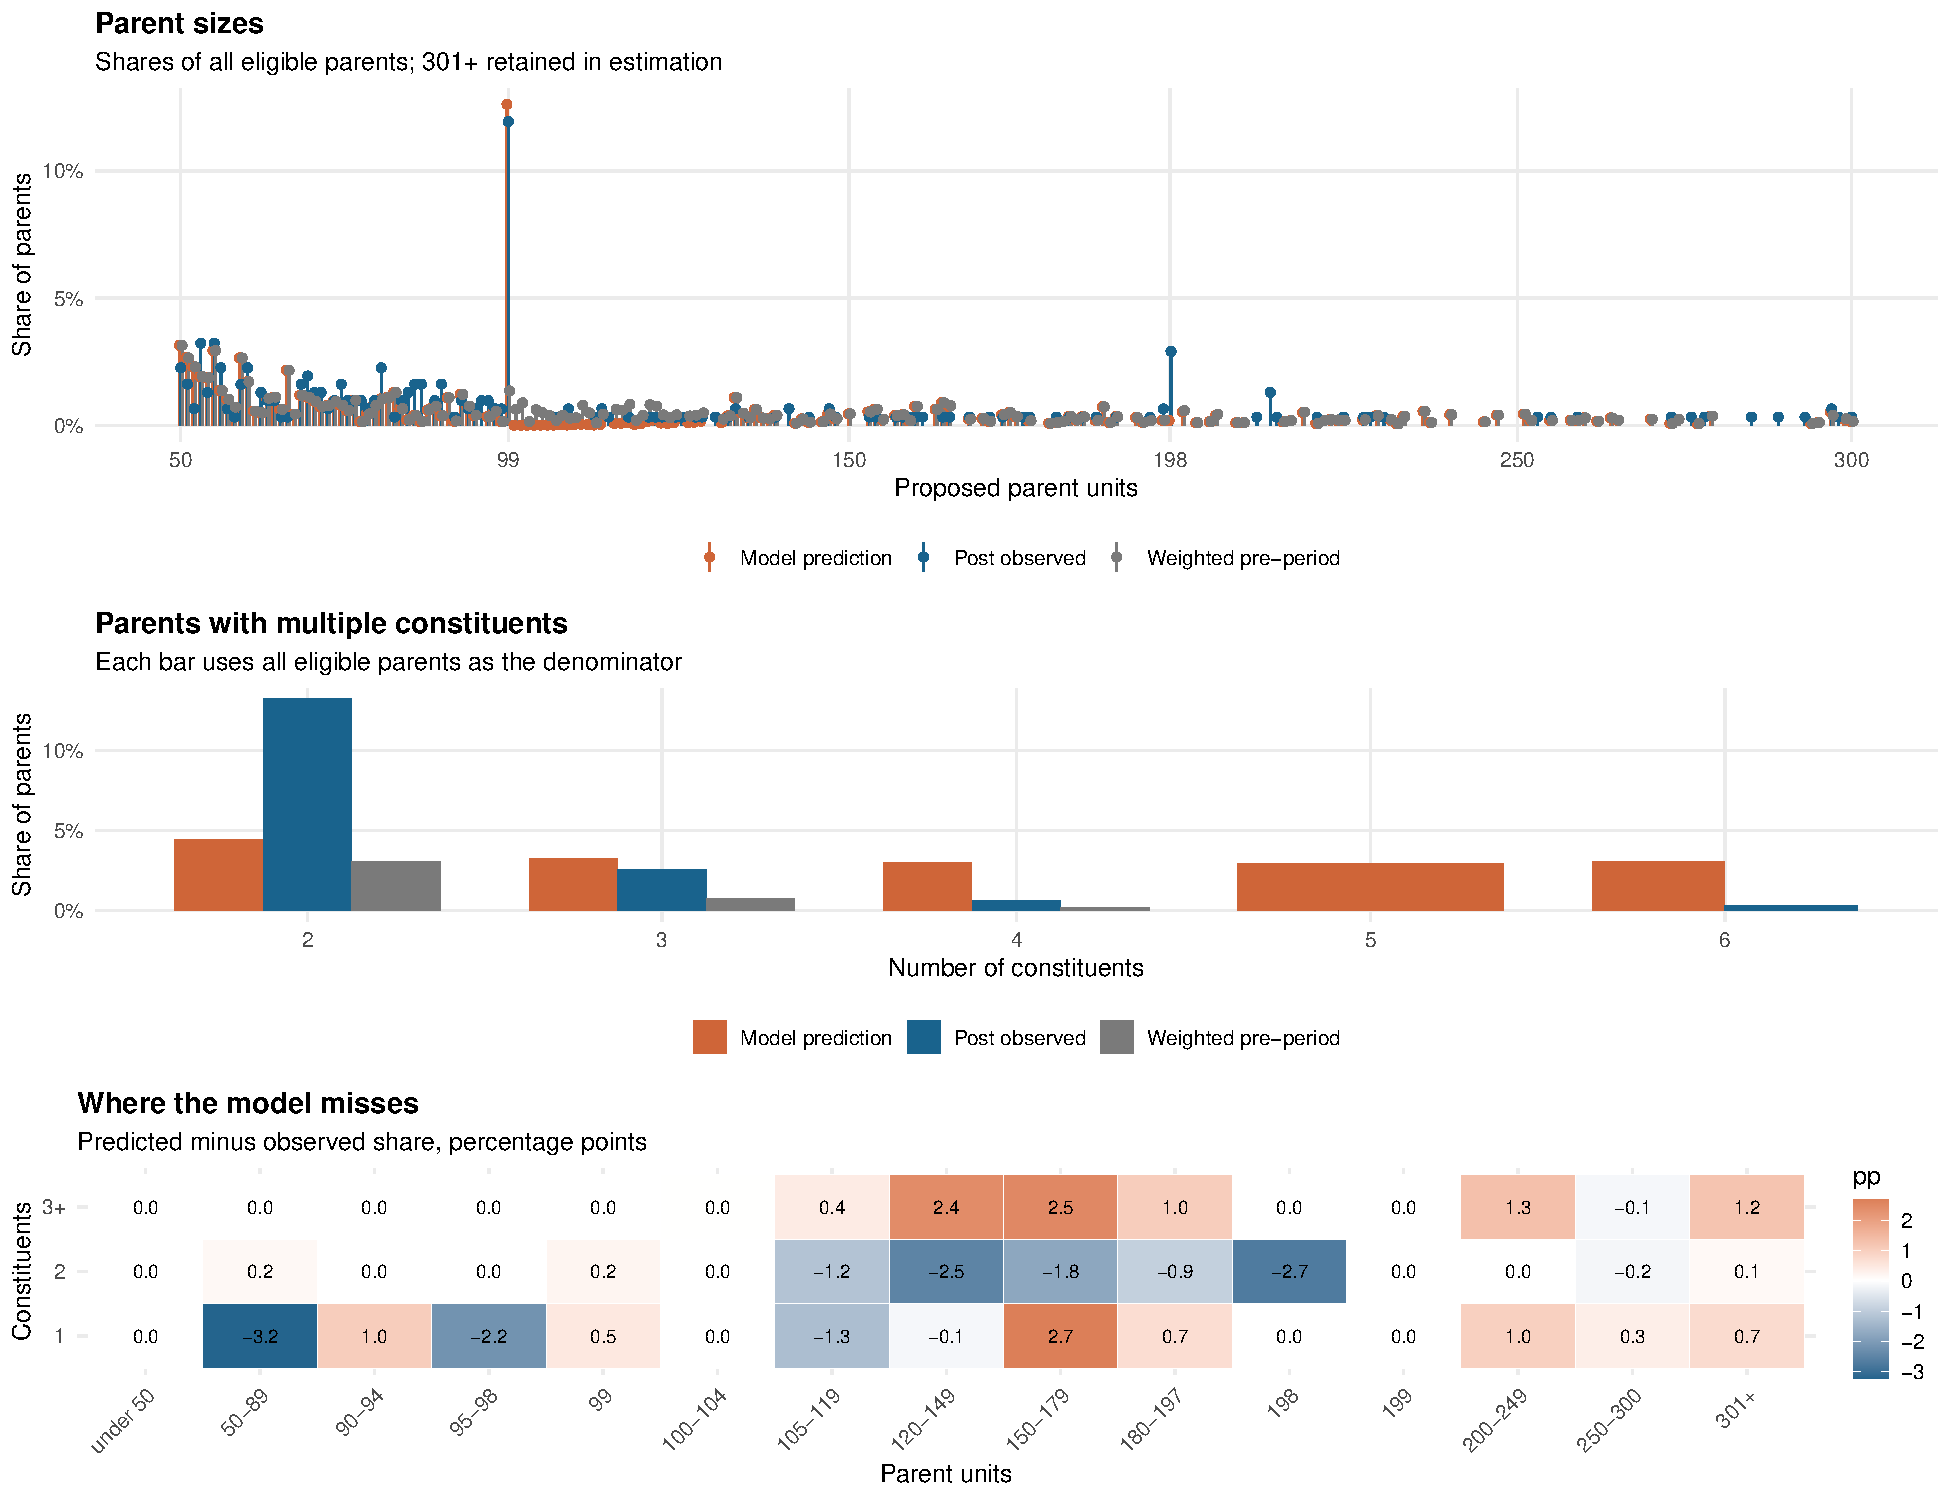
\includegraphics[width=\textwidth]{archive/2026-09-22-prepolicy-pilot/pdf/fit_overview.pdf}
\end{center}

Thirteen numerical checks pass, including exhaustive integer size searches,
an independent partition dynamic program, and organization probabilities checked
against simulation. Two known parameter pairs are recovered uniquely from exact
synthetic moments. Ten finite samples per pair reveal substantial variation.
Deleting each of the eight observed 100--119-unit parents individually leaves
the baseline minimizer unchanged. Structural uncertainty from estimating the
historical weights remains to be evaluated.

Joint assessment leaves ordinary organization unchanged and fits worse.
Curvature and seven-constituent sensitivities also underpredict $99+99$ parents.
These are mechanical single-100-unit schedules; the geographic 150-unit regime
and verified legal assessment units require further modeling. The full model
framework retains its general cost specification.

\textit{Reproduction note.} Run \texttt{make pure-notch-pilot} from the repository
root. The audit README records the grids, assumptions, and output definitions;
\texttt{parameter\_grid.csv} retains every fit and its quantities.
Source-file fingerprints are in \texttt{input\_provenance.csv}.
This run uses the working-tree research changes following revision
\texttt{a665b53}, with R 4.5.2 and GNU Make 3.81.

\clearpage
\subsection*{Follow-up: Does adding multi-lot status improve the fit?}

Adding the archival multi-lot indicator to the calibration improves the
two-filing share but worsens the overall joint fit. This sensitivity uses
the same 561 historical parents, 316 post parents, model assumptions,
45 cells, and 572 parameter combinations as the baseline search.

\begin{center}
\small
\begin{tabular}{lrrr}
\hline
Outcome & Observed & Baseline fit & Multi-lot weights \\
\hline
Parents at 99 units (\%) & 12.34 & 12.78 & 13.02 \\
Exactly two filings (\%) & 12.66 & 3.94 & 9.57 \\
Three or more filings (\%) & 3.48 & 11.61 & 9.89 \\
Parents organized as $99+99$ (\%) & 2.85 & 0.17 & 0.12 \\
Mean proposed units & 138.63 & 148.96 & 155.98 \\
\hline
\end{tabular}
\end{center}

The best alternative grid point is $\kappa=0.115$ and
$\sigma_{\mathrm{org}}=1.6$. Total squared joint-share error rises from
0.005675 to 0.007562, an increase of 33.3 percent. The alternative implies
527 fewer units, compared with 520 in the baseline, while the difference
between its historical counterfactual and observed post totals grows from
3,783 to 6,009 units.
The largest deterioration is the 50--89-unit single-filing cell: its observed
share is 46.5 percent, while predictions fall from 43.7 to 41.4 percent.
The total pair share is closer, but squared errors across pair-size cells
also increase, with excess weight on very small and large pairs.

The improvement in pairs comes mainly from changing the counterfactual
organization distribution. Historical two-filing parents receive 8.97 percent
of weight with the multi-lot moment, compared with 2.56 percent without it.
The total historical share with multiple filings rises from 3.46 to 10.53
percent. More observed organization can consequently be attributed to ordinary
development. The alternative still produces too many three-plus parents and
almost none of the observed $99+99$ concentration.

The indicator counts distinct archival parcels matched to the parent site.
Post-period parcels come from the fixed 2023 map; historical parcels use
filing-specific lagged maps. Under Jacob's given-footprint assumption,
archival parcel structure is a plausible site characteristic to balance.
The relevant research choice is whether that matched parcel set belongs to
the given site or reflects development choices whose response is being studied.
The observed parent grouping determines which archival lots are combined,
so a pre-policy map alone does not settle that interpretation. The adopted
calibration remains unchanged.

\textit{Reproduction note.} The same \texttt{make pure-notch-pilot} command
now builds this sensitivity. The comparison script reproduces the saved
baseline weights before adding the extra moment. Positive alternative weights
have effective sample size 408.6 and maximum matched-total error
$8.36\times10^{-9}$. The four \texttt{multilot\_*} CSV outputs preserve
parent weights, every searched fit, outcome comparisons, and objective
components by constituent count. Standard reports are written with these data.

\clearpage
\subsection*{Follow-up: Which parent sizes account for the unit gap?}

Parents above 300 units contribute 3,110 units, or 82.2 percent, of the net
historical-to-post difference. This comparison scales the adopted weighted
historical distribution to the 316 observed post parents. Its total is 47,590
proposed units, compared with 43,807 observed, giving
\[
316\times(150.6016-138.6297)\simeq 3{,}783.1.
\]
Each bar below sums exact units within that period's observed size bin.
Positive bars indicate more units in the historical benchmark; negative bars
indicate more units observed after the policy.

\begin{center}
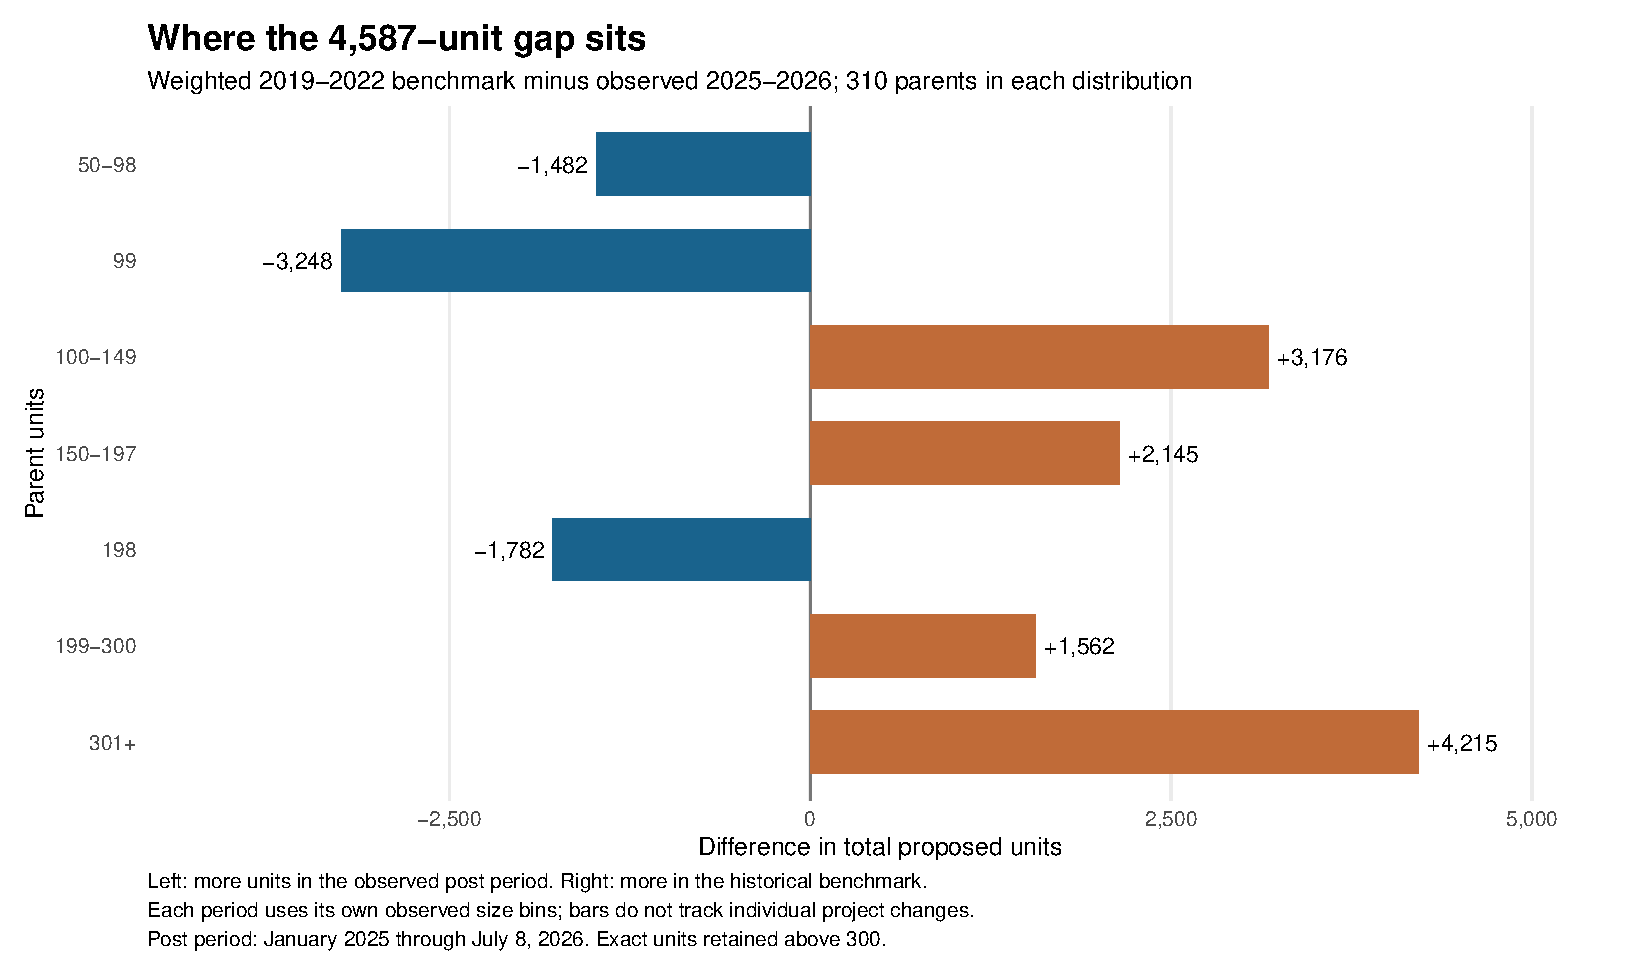
\includegraphics[width=\textwidth]{archive/2026-09-22-prepolicy-pilot/pdf/unit_gap_by_size.pdf}
\end{center}

The historical benchmark contains 30.89 parents above 300 units, compared with
25 observed. Their mean sizes are nearly equal: 512.10 and 508.36. Valuing the
5.89-parent difference at the observed tail mean gives 2,994 units; differing
tail means account for the remaining 115. This accounting does not follow
individual developments. A project shrinking from 320 to 198 units would also
reduce the upper-tail count. Compression and changes in the project mix remain
possible explanations. The smaller bins contain substantial offsetting changes,
including excess post units at exactly 99 and 198.

Jacob requested discussion of this gap before further estimation. The planned
sequence retains the adopted sample, weights, and 45 fitting cells: first fit
increasing organization costs with the flat charge, then try linear and quadratic
one-parameter burdens. This decomposition leaves the fitted model unchanged.

\textit{Reproduction note.} \texttt{make pure-notch-pilot} runs
\texttt{decompose\_unit\_gap.R} from the saved pilot parent sample. The resulting
\texttt{unit\_gap\_by\_size.csv} records actual historical counts, weighted
equivalent counts, observed counts, exact unit totals, and within-bin means.
The seven display bins aggregate sizes independently of the fitting cells.

\clearpage
\subsection*{Follow-up: Splitting among parents with three or more filings}

Ten of the eleven post-period parents with at least three filings have every
constituent below 100 units. Five contain multiple exact 99s, including two
triples, one quadruple, and a six-filing parent with five 99s plus 96. Jacob
requested this inspection before setting aside information from larger parents.

\begin{center}
\small
\begin{tabular}{llr}
\hline
Parent streets & Constituent units & Total \\
\hline
Pacific / Dean, Brooklyn & $82+82+64$ & 228 \\
Beach 29th / 30th, Queens & $99+74+57$ & 230 \\
38th Avenue / 32nd / 33rd, Queens & $87+84+82$ & 253 \\
Walton / East Burnside, Bronx & $94+84+77$ & 255 \\
Myrtle / Wyckoff, Queens & $99+98+92$ & 289 \\
4121 / 4133 / 4137 Third, Bronx & $99+99+99$ & 297 \\
Bruckner / Brook / East 132nd, Bronx & $99+99+99$ & 297 \\
Wyckoff / Bergen, Brooklyn & $99+99+99+70$ & 367 \\
Sullivan / Empire, Brooklyn & $99+99+99+99$ & 396 \\
89-01--89-53 165th Street, Queens & $99+99+99+99+99+96$ & 591 \\
West / Freeman, Brooklyn & $526+287+210$ & 1,023 \\
\hline
\end{tabular}
\end{center}

All five repeated-99 parents exceed 249 units. Three remain above 300 even
though each constituent is below 100. A local objective restricted to parent
totals of 50--249 would omit all five; extending to 300 would retain the two
triples but still omit the quadruple and six-filing patterns. The recommendation
is to preserve this organization information when choosing which moments to fit.
The seven historical parents with at least three filings contain no exact 99s.

These vectors support investigating policy-related organization beyond 198.
They do not identify any parent's counterfactual size or quantify its contribution
to the upper-tail unit shortfall. A 297-unit triple could have shrunk from above
300, but the vector alone cannot establish that. Conversely, the 367-, 396-, and
591-unit parents already contribute to the observed upper tail. Their splitting
patterns show why a modest tail-count difference can coexist with a substantial
organization response. Even an absence of repeated 99s would not establish that
the entire size gap reflects changes in the project mix.

The below-100 flags describe the pilot's separate-assessment rule. Existing
verification records classify Wyckoff/Bergen as verified separate 485-x units,
Third Avenue, Bruckner, and Sullivan/Empire as suggestive, and 165th Street as
unable to verify. An economic parent and a below-100 vector alone do not establish
legal exemption. Administrative unit priority and reviewed link decisions remain
in force; this inspection makes no sample or model changes.

\textit{Reproduction note.} \texttt{make pure-notch-pilot} now also writes
\texttt{post\_three\_plus\_parents.csv} from the saved pilot sample, with full
addresses, vectors, threshold counts, and coverage flags. All eleven vectors,
component counts, and totals were checked against 38 unique additive filings
in the canonical constituent panel. The existing gap producer writes the
table and its standard data report.

\clearpage
\subsection*{Follow-up: A local unit quantity with tail uncertainty}

Jacob requested a unit quantity centered on counterfactual parent sizes up to
250, with larger parents retained in the organization fit. At the existing
flat-charge estimates, the implied reduction is approximately 513 units from
counterfactual sizes of 50--250 and 7 units from larger origins, summing to the
pilot's 520 units. The calculation is $316\sum_i\sum_J w_i p_{iJ}(x_i-m_{iJ})$,
restricted by counterfactual $x_i$. All simulated parents, adopted weights, and
45 fitting cells are retained. In particular, organization among larger parents
still enters the objective. The cutoff of 250 is an exploratory reporting
choice; it does not assert that all policy effects end there.

With the fitted $\kappa=0.11$, the fixed-organization flat-charge condition is
$x\leq 99J+99\sqrt{\kappa}$. The resulting upper sizes are 131.84 for one filing
and 230.84 for two. Assigning the 34.76 excess parents at 99 uniformly to integer
origins 100--131, and nine excess parents at 198 to 199--230, gives an average
reduction of 16.5 units in each group. This produces about 574 plus 149, or
722 units. That calculation assumes origins and attributes all excess mass to
policy. It is an illustration, not an estimated causal quantity or a bound.
The structural pilot uses the weighted historical distribution and organization
costs and continues to underpredict pairs of 99. Compression under growing
burdens and sampling uncertainty in the fitted local effect remain unestimated.

The tail-count difference is 5.89 parent equivalents, with a 95 percent percentile
bootstrap interval of approximately $[-4.2,16.9]$. The existing bootstrap
resamples historical and post parents separately, holds sample sizes fixed,
and recalibrates site weights. The interval uses 489 successful calibrations
out of 499 attempts. It treats parents as independent and does not account for
link uncertainty or common developer shocks. This supports reporting the tail
as a non-attributed distribution difference rather than requiring the model to
explain its 3,110-unit contribution to the aggregate gap.

The claim that leaving the upper tail requires shrinking to 198 does not hold
with three filings. A 320-to-297 change costs $((320-297)/99)^2\simeq0.054A$,
compared with $1.519A$ for 320-to-198. The existing model predicts 0.332 parent
equivalents leaving the 301+ bin, all to 297. The observed triples therefore
matter for the mechanism even though they do not identify their counterfactual
sizes. Larger-parent responses under growing burdens require estimation.

\href{https://www.nyc.gov/site/hpd/services-and-information/tax-incentives-421-a.page}{HPD}
records June 15, 2022 as the 421-a construction-commencement deadline. In the
selected historical filing sample, the shares above 300 units are 11.2 percent
in 2019, 14.0 percent in 2020, 20.3 percent in 2021, and 9.5 percent in 2022.
The highest share is in 2021. A filing date is not a foundation-commencement
date, so these records do not establish how much of the historical tail reflects
anticipation of the deadline. The expiration-rush explanation remains a
counterfactual-composition hypothesis.

\textit{Reproduction note.} Run \texttt{make pure-notch-pilot}.
The four CSV outputs record local model quantities, illustrative bunching arithmetic, tail-count
intervals, and historical filing-year composition, with standard reports.
The point estimates in the bootstrap inputs are checked against the pilot
sample and weights. The model and fitting window are unchanged.

\clearpage
\subsection*{Follow-up: Parcel structure of the five repeated-99 parents}

The five repeated-99 parents contain 20 distinct DOB building identifiers and
1,948 proposed units. Four have recorded instruments describing one zoning lot
containing multiple existing or tentative tax lots. The parcel review also
finds incomplete historical land coverage for three parents.

\begin{center}
\small
\begin{tabular}{lrrrr}
\hline
Parent & Filings & Matched old lots & Matched area & Associated old area \\
\hline
Wyckoff/Bergen & 4 & 1 & 46,692 & 50,692 \\
Sullivan/Empire & 4 & 1 & 38,118 & 38,118 \\
165th Street & 6 & 3 & 23,280 & 111,540* \\
Third Avenue & 3 & 3 & 19,555 & 22,139 \\
Bruckner/Brook/E132 & 3 & 3 & 28,700 & 28,700 \\
\hline
\end{tabular}
\end{center}
Areas are square feet from 2023 PLUTO. The reviewed sets contain 3, 1, 8, 4,
and 3 old parcels. *The eight associated 165th Street parcels are not yet a
verified usable footprint of the six-building proposal.

The \href{https://extapps.dec.ny.gov/data/DecDocs/C224403/Agreement.BCP.C224403.2025-08-15.Amendment_No1_Change_Owner_Modify_Description.pdf}{Wyckoff/Bergen DEC amendment}
identifies old lots 19/42/51 becoming 19/20/21/57. Production recovers only
lot 19, omitting two 2,000-square-foot parcels. Its January 2025 ACRIS statement
calls the four tentative parcels one zoning lot. At Sullivan/Empire, a
\href{https://a836-acris.nyc.gov/DS/DocumentSearch/DocumentDetail?doc_id=2026030900544002}{March 2026 statement}
describes old lot 28 becoming four tentative tax lots within one zoning lot.
PLUTO 26v2 still shows only lot 28. A cap of one filing per old tax lot would
exclude both observed proposals.

At Third Avenue, the July 2025 OER work plan identifies old lots 27/30 being
merged into tentative lot 27. The old site contains 27/30/31/35; production
misses lot 30. An \href{https://a836-acris.nyc.gov/DS/DocumentSearch/DocumentDetail?doc_id=2026042300841002}{April 2026 declaration}
treats the three new lots as one zoning lot. At Bruckner, a
\href{https://a836-acris.nyc.gov/DS/DocumentSearch/DocumentDetail?doc_id=2026070900534002}{July 2026 statement}
describes one zoning lot but changes the internal boundaries while retaining
lot numbers 1/34/38. Recorded July 10, it is follow-up evidence after the
July 8 sample endpoint.

Four 165th Street jobs use condominium billing lot 7501. Its
\href{https://a836-acris.nyc.gov/DS/DocumentSearch/DocumentDetail?doc_id=2024081600593001}{2024 declaration}
names six predecessor parcels; production maps all four jobs to old lot 30.
With the two other filing lots, the associated parcels cover 111,540 square
feet. The declaration describes commercial property with two condominium
units. Subsequent termination instruments and current PLUTO document further
changes. A plan crosswalk must establish the development footprint and retained
uses before substituting a larger area. Current zoning-lot and HPD application
arrangements remain unresolved.

\href{https://www.nysenate.gov/legislation/laws/RPT/485-X}{RPTL 485-x}
defines an eligible site using a tax lot or a zoning lot containing multiple
dwellings within one ANNY benefits application. DOB jobs and tax lots do not
by themselves establish separate wage assessment. Wyckoff/Bergen's registrations
report separate sub-100 buildings, providing evidence of intended registration;
final assessment remains unverified. PLUTO has no zoning-lot ID, and SplitZone
indicates boundaries between zoning districts or overlays.

Codex recommends a given outer land footprint with internal subdivision and
building count chosen by the developer. Corrected area, dimensions, zoning,
and parcel history can inform feasibility and organization costs. Final
subdivisions are outcomes. The current pilot assigns one independent cost draw
to each alternative J; per-added-filing costs require re-estimation. The observed
stacks alone cannot identify counterfactual units or units preserved by splitting.

\textit{Reproduction note.} Run \texttt{make pure-notch-pilot}. Four parcel
outputs reconcile to the canonical filings and production areas. The existing
acquisition audit holds dated PLUTO/ACRIS snapshots, queries, and hashes; two
cited audit tables preserve documentary reading. Production panels and weights
await the identified parcel corrections; unit vectors and model definitions
are unchanged.
